% ----------------------------------------------------------------------- %
% Master Thesis Template for M.Tech Programme, VIT Vellore Campus
% Tex document prepared by Dr. SUDHAKAR. P, Dr. UMA PRIYA D and Dr. MALINI S
% Version 00.01 published on : 17-10-2025
% ----------------------------------------------------------------------------- %
% import necessary packages
\documentclass[12pt, english, onehalfspacing]{report}
\usepackage{graphicx} % Required for inserting images
\usepackage{geometry}
\usepackage{ragged2e}
\usepackage{titlesec}
%\usepackage{natbib}
\usepackage{array}
\usepackage{lipsum}
\usepackage{setspace}
\usepackage{tikz}
\usepackage{pgfplots}
\usepackage{subcaption}
\usepackage{etoolbox}
\usepackage{nomencl}
\makenomenclature
\usepackage{parskip}
\usepackage{listings}
%\usepackage[backend=biber,style=authoryear]{biblatex}
%\addbibresource{mali.bib}
\renewcommand{\familydefault}{\sfdefault}

\pretocmd{\chapter}{\justifying}{}{}

%\usepackage{draftwatermark}
%\SetWatermarkText{DRAFT 1.0}
%\SetWatermarkScale{0.4}

% Font: Times New Roman
\usepackage{newtxtext,newtxmath}

% Line spacing
\usepackage{setspace}
\setstretch{1.5}   % 1.5 spacing

% Margins
%\usepackage[a4paper,top=50mm,bottom=25mm,left=30mm,right=25mm]{geometry}

% Section formatting
\usepackage{titlesec}

% Chapter format: "Chapter 1" + Title
\DeclareRobustCommand{\chaptertitleformat}[1]{\MakeUppercase{#1}}

\titleformat{\chapter}[display]
  {\normalfont\bfseries\fontsize{14pt}{16pt}\selectfont}
  {\centering Chapter \thechapter}
  {0pt}
  {\centering\bfseries\fontsize{16pt}{18pt}\selectfont\chaptertitleformat}

% Section: 14pt, Title Case, Bold
\titleformat{\section}
  {\normalfont\bfseries\fontsize{14pt}{16pt}\selectfont}
  {\thesection}{1em}{}

% Subsection: 12pt, Sentence case
\titleformat{\subsection}
  {\normalfont\fontsize{12pt}{14pt}\selectfont}
  {\thesubsection}{1em}{}

% Subsubsection: 12pt, Sentence case
\titleformat{\subsubsection}
  {\normalfont\fontsize{12pt}{14pt}\selectfont}
  {\thesubsubsection}{1em}{}

% Captions for figures/tables (TNR, 11pt)
\usepackage[font=small,labelfont=bf]{caption}
\captionsetup{font={rm,footnotesize}} % ~11pt equivalent

% Tables: ragged right alignment option
\usepackage{array}
\newcolumntype{R}[1]{>{\RaggedRight\arraybackslash}p{#1}}

% For figures
\usepackage{graphicx}

\usepackage{nomencl}
\renewcommand{\nomname}{}
\renewcommand{\nomlabel}[1]{#1 \hfill}
\makenomenclature

%To control spacing above a new \paragraph

%-------------------------------------------------------------------%	
%            MARGIN SETTINGS  (Do not change!)
%-------------------------------------------------------------------
\geometry{
	paper=a4paper, % Change to letterpaper for US letter
	inner=2.5cm, % Inner margin
	outer=2.0 cm, % Outer margin
	bindingoffset=.5cm, % Binding offset
	top=1.5cm, % Top margin
	bottom=1.5cm, % Bottom margin
	%showframe, % Uncomment to show how the type block is set on the page
}

%-------------------------------------------------------------------%	
%           Thesis configurations (Enter your information here
%-------------------------------------------------------------------


\newcommand{\thesistitle}{Thesis title} % 
\newcommand{\studentname}{Student name}
\newcommand{\studentregno}{RegNo}
\newcommand{\projsupervisor}{Dr. Project guide name}
\newcommand{\projsupervisordesignation}{designation}
\newcommand{\projsupervisorschool}{School of Computer Science and Engineering}
\newcommand{\projstartdate}{dd-mm-yyyy} 
\newcommand{\projenddate}{dd-mm-yyyy}
\newcommand{\hodname}{Dr. HoD name}
\newcommand{\hoddept}{HoD Department}
\newcommand{\specialization}{Programme specialization}
\newcommand{\thesisdate}{dd-mm-yyyy} % thesis submission date
\newcommand{\thesismonth}{Month}
\newcommand{\thesisyear}{Year}
%-------------------------------------------------------------------

\renewcommand{\nomlabel}[1]{#1 \hfill}

% Group headings
\renewcommand{\nomgroup}[1]{%
   \item [\bfseries 
   \ifstrequal{#1}{A}{\Large\textbf{List of Abbreviations}}{% 
   \ifstrequal{#1}{S}{\Large\textbf{List of Symbols}}}% 
   %\ifthenelse{\equal{#1}{A}}{\item[\Large\textbf{List of Abbreviations}]}{%
   %\ifthenelse{\equal{#1}{S}}{\item[\Large\textbf{List of Symbols}]}}%
]}%

%--------------------  Thesis front matter     ----------------------------------------- 
\begin{document}
\pagestyle{plain}
\pagenumbering{roman}
\addtocounter{page}{-1}
\thispagestyle{empty}
\centering 
\vspace{1cm}
\large{ \textbf{INTERNSHIP I / DISSERTATION I REPORT}} \linebreak
 \linebreak
\normalsize{\textit{Submitted in partial fulfilment of the requirements for the degree of}} \linebreak
\vspace{1em} \linebreak
\large{\textbf{M.Tech. Computer Science and Engineering}}\\(\textbf{\specialization}) \linebreak
\vspace{0.5cm} \linebreak
by \linebreak 
\vspace{0.5em} \linebreak
\Large{\textbf{\studentname}} \linebreak
\large{\textbf{\studentregno}} \linebreak
\vspace{1cm} \linebreak
\normalsize{Under the Supervision of} \linebreak 
\vspace{0.5em} \linebreak
\Large{\textbf{\projsupervisor}} \linebreak 
\normalsize{\projsupervisordesignation} \linebreak
\vspace{2cm}
\begin{figure}[!h]
	\centering
	\includegraphics[scale=1]{./images/vit\_logo.png}
\end{figure}
\linebreak \vspace{1cm}
\large{\textbf{SCHOOL OF COMPUTER SCIENCE AND ENGINEERING}} 
\linebreak \vspace{0.5cm}
\textbf{\thesismonth, \thesisyear}
\pagebreak
\centering
\begin{center}
	\Large{DECLARATION}	
\end{center}
\vspace{1em}
\normalsize
 
\begin{flushleft}
\justifying
I, \textbf{\studentname \;(\studentregno)} hereby declare that the thesis entitled \textbf{``\thesistitle''} submitted to Vellore Institute of Technology (VIT), Vellore for the award of the degree of \textbf{Master of Technology in Computer Science and Engineering (\specialization)} is a record of bonafide work carried out by me under the supervision of \textbf{\projsupervisor}, {\projsupervisorschool}, Vellore Institute of Technology, Vellore. \par

I further declare that the work reported in this project report has not been submitted and will not be submitted, either in part or in full, for the award of any other degree or diploma in this institute or any other institute or university.
\end{flushleft}
\paragraph{}
\vspace{5cm}

\noindent Place: Vellore \hspace{8cm} Signature of the Candidate \linebreak
\noindent Date: \thesisdate \hspace{11.5cm} \linebreak
\pagebreak

\centering
\begin{center}
	\Large{CERTIFICATE}	
\end{center}
\vspace{1em}
\normalsize
\justifying
\begin{flushleft}
\justifying
This is to certify that the thesis entitled \textbf{``\thesistitle ''} submitted by \textbf{\studentname \; (\studentregno)}, School of Computer Science and Engineering, Vellore Institute of Technology, Vellore for the award of the degree of \textbf{Master of Technology in Computer Science and Engineering (\specialization)}, is a record of bonafide work carried out by him/her under my supervision during the period, \textbf{\projstartdate} to \textbf{\projenddate} as per the VIT code of academic and research ethics. \par

The contents of this report have not been submitted and will not be submitted either in part or in full, for the award of any other degree or diploma in this institute or any other Institute or University. The dissertation fulfills the requirements and regulations of the Institute and in my opinion meets the necessary standards for submission.	
\end{flushleft}
\paragraph{} 
\vspace{5cm}

%\raggedright
\begin{flushleft}
    Place: Vellore, \hspace{7.5cm} Name and signature of the guide \linebreak
Date: \thesisdate \hspace{10.5cm} \linebreak
\end{flushleft}
\par
\vspace{4em} 
\textbf{Internal Examiner} \hspace{7.5cm} \textbf{External Examiner} \linebreak
\vspace{4em}
\begin{center}
	\textbf{Head of the Department} \linebreak
	\textbf{Department of \hoddept}
\end{center}
\pagebreak

\centering
\begin{center}
	\Large{It should be produced with company letter head}	
\end{center}
\vspace{1em}
\raggedleft
Date : .................
\linebreak \vspace{1em}
\begin{center}
	\Large{CERTIFICATE BY THE EXTERNAL GUIDE}	
\end{center}

\begin{flushleft}
\justifying
This is to certify that the project entitled \textbf{``\thesistitle''} submitted by \textbf{\studentname \; (\studentregno)} to Vellore Institute of Technology  in partial fulfillment of the requirement for the award of the degree of  \textbf{Master of Technology in Computer Science and Engineering (\specialization)} is a record of bonafide work carried out by him/her under my guidance during the period, \textbf{\projstartdate} to \textbf{\projenddate}.  The project fulfills the requirements as per the regulations of this Institute and in my opinion meets the necessary standards for submission.   The contents of this report have not been submitted and will not be submitted either in part or in full, for the award of any other degree or diploma in this institute or any other institute or university.	
\end{flushleft}
\paragraph{}
% \normalsize{Signature of the External Supervisor} \\
\vspace{1cm}
Name, \\
\vspace{1cm}
%--------------- Configure External supervisor information here -------------
\large{EXTERNAL SUPERVISOR} \\
(title ) \\
(Full address of the Institution / organization) \\
(e-mail id, phone no) \\
(Seal of the Institution / Organization)
\pagebreak
 % comment if necessary
\centering
\begin{center}
	\Large{ABSTRACT}	
\end{center}
\vspace{1em}
\normalsize
 
%------------ Change this paragraph and add your executive summary ---------------
\begin{flushleft}
\justifying	
Summary should be a one page synopsis of the thesis typed with “Times New Roman” font of size 12. Abstract must be typeset with 1.5 line spacing. It is a brief summary of the thesis content. It should be of maximum one page long. It can best describe the problem addressed in the thesis. In summary, it can describe the completed work along with the findings or lessons learned, if any. The keywords mentioned below must be in italics. \par
\noindent \textit{\textbf{Keywords:} Thesis, Dissertation, Degree, Sample Thesis, Literature.}
\end{flushleft}
\pagebreak

\centering
\begin{center}
\Large{ACKNOWLEDGEMENTS}
\end{center}
\vspace{1em}
\normalsize
\justifying
\begin{flushleft}
\justifying
\par With immense pleasure and a deep sense of gratitude, I wish to express my sincere thanks to my supervisor \textbf{Dr. K. Anil Kumar}, School of Computer Science and Engineering, Vellore Institute of Technology (VIT), Vellore without his/her motivation and continuous encouragement, this research would not have been successfully completed.	 

\par I am grateful to the Chancellor of VIT, \textbf{Dr. G. Viswanathan}, the Vice Presidents, and the Vice Chancellor for motivating me to carry out research in the Vellore Institute of Technology. 

\par It would be no exaggeration to say that the Dean in-charge of SCOPE, \textbf{Prof. Jaisankar N}, was always available to clarify any queries and clear the doubts I had during the course of my project.
I would also like to acknowledge the role of the HoD, \textbf{Dr. G. Swati Jain}, who was instrumental in keeping me updated with all necessary formalities and posting all the required formats and document templates through the mail, which I was glad to have had. 

\par Finally, I would like to thank \textbf{Vellore Institute of Technology} for providing me with infrastructural facilities, a flexible choice and for supporting my research and execution related to the dissertation work.
\end{flushleft}
\paragraph{} 
\vspace{3cm}

\begin{flushleft}
Place: Vellore, \hspace{6cm} \textbf{Bollu Sai Likhitha \; (24MAI0083)} \linebreak
Date: 06-11-2025 \hspace{8cm} \linebreak    
\end{flushleft}

\pagebreak


%-----------------------------------------------------------------
% Table of content to be included 
% List of figures
% Symbols and Abbreviations
\tableofcontents
\newpage
\listoffigures
\newpage
\listoftables
\newpage

\nomenclature[A]{\(AI\)}{Artificial Intelligence}
\nomenclature[A]{\(ML\)}{Machine Learning}
\nomenclature[S]{\(a\)}{Acceleration (m/s$^2$)}
\nomenclature[S]{\(v\)}{Velocity (m/s)}
\printnomenclature
\newpage

%--------  Thesis contents -----------------------------------
\pagenumbering{arabic}
\setcounter{page}{1}
\chapter{\uppercase{INTRODUCTION}}

\section{Overview}

\section{Objectives}

The format for typing Chapter headings, section headings and sub-section headings are explained by the following illustrative examples.

\subsubsection{Chapter Heading Example}
Chapter heading: Chapter 1 INTRODUCTION

\subsubsection{Section Heading Example}
Section heading: 1.1 Outline of Thesis

\subsubsection{Subsection Heading Example}
Sub-section heading: 1.1.1 Literature review

\subsubsection{Sub-subsection Heading Example}
Sub-subsection heading: 1.1.1.1 Synthetic aperture radars on satellites

The word \textbf{Chapter} without punctuation should be centered 50 mm down from the top of the page. Two spaces below, the title of the chapter should be typed in capital letters. Moreover, the title should be center aligned. The text should commence 2 spaces below this title, the first letter of the text starting 20 mm inside from the left-hand margin. The section and sub-section captions along with their numbering should be left justified. The typed material directly below section or sub-section heading should commence 1.5 space below it \cite{alishahi2009bounds}, \cite{hawley2004handbook}, \cite{conley1998nativity}, \cite{doan2002learning}. 

\begin{itemize}
    \item Chapter number: 14, Regular, Times New Roman, bold
    \item Chapter Heading Font Size: 16, Regular, Times New Roman, CAPS, bold
    \item Section Heading Font Size: 14, Times New Roman, Title Case, bold
    \item Subsection Heading Font Size: 12, Regular, Times New Roman, Sentence case
    \item Subsubsection Heading Font Size: 12, Regular, Times New Roman, Sentence case
\end{itemize}
\chapter{\uppercase{Literature Review}}
\section{Review of Literature}
A literature review is a text of a scholarly paper, which contains the current knowledge 
including substantive findings, as well as theoretical and methodological contributions to 
a particular topic. Literature reviews are secondary sources, and do not report new or 
original experimental work. Most often associated with academic-oriented literature, 
such reviews are found in academic journals, and are not to be confused with book reviews 
that may also appear in the same publication. Literature reviews are a basis for research 
in nearly every academic field (Waldron, 2008b). 

A narrow-scope literature review may be included as part of a peer-reviewed journal article 
presenting new research, serving to situate the current study within the body of the relevant 
literature and to provide context for the reader. In such a case, the review usually precedes 
the methodology and results sections of the work. Producing a literature review may also be 
part of graduate and post-graduate student work, including in the preparation of a thesis, 
dissertation, or a journal article. Literature reviews are also common in a research proposal 
or prospectus (the document that is approved before a student formally begins a dissertation 
or thesis) (Doan et al., 2002; Duzdevich et al., 2014; Ganesh et al., 2016).

\section{Review Types}
The main types of literature reviews are: evaluative, exploratory, and instrumental 
(Duzdevich et al., 2014; Neil and David, 2016). 

A fourth type, the systematic review, is often classified separately, but is essentially a 
literature review focused on a research question, trying to identify, appraise, select and 
synthesize all high-quality research evidence and arguments relevant to that question. 
A meta-analysis is typically a systematic review using statistical methods to effectively 
combine the data used on all selected studies to produce a more reliable result \cite{duzdevich2014dna}, \cite{mohanaprasad2017optimized}, \cite{gilbarg1977elliptic}, \cite{haykin2004kalman}, \cite{haykin2005cognitive}, \cite{knuth1986computers}.

\subsection{Process and Product}
Gilbarg and Trudinger (2015) distinguish between the process of reviewing the literature 
and a product known as a literature review. The process of reviewing the literature is 
often ongoing and informs many aspects of the empirical research project.

\section{Page Limit of Review}
A careful literature review is usually between 8 to 20 pages. The process of reviewing 
the literature requires different kinds of activities and ways of thinking. 
(Duzdevich et al., 2014) and (Kothari, 2004) link the activities of doing a literature review 
with Benjamin Bloom’s revised taxonomy of the cognitive domain (ways of thinking, 
remembering, understanding, applying, analysing, evaluating, and creating).
\chapter{\uppercase{Problem Description}}

\section{Problem Description}
A critical section that clearly explains the issue or gap your research aims to address. It sets the foundation for the entire study. A strong problem description include

\begin{itemize}
	\item Context or Background
	\item The Gap
	\item Specific problem 
	\item Significance to solve it
\end{itemize}
\subsection{Dataset Description}
A dataset is a collection of related data that is organized and formatted in a specific structure, typically used for analysis, research, or training machine learning models. Discuss about your dataset and its characteristics.
 % included 
\chapter{\uppercase{Proposed Approach}}

%\onehalfspacing % 1.5 line spacing

% -----------------------------
% Table 3.1
% -----------------------------
\begin{table}[h!]
\centering
\caption{Country list}
\renewcommand{\arraystretch}{1.3} % Row height
\begin{tabular}{|l|l|l|l|}
\hline
\textbf{Country/Area Name} & \textbf{Description} & \textbf{ISO alpha 3 Code} & \textbf{ISO numeric Code} \\
\hline
Afghanistan & It is a Country & AFG & 004 \\
Aland Islands & It is an Island & ALA & 248 \\
Albania & It is a small city & ALB & 008 \\
Algeria & It is a Country & DZA & 012 \\
American Samoa & It is a Country & ASM & 016 \\
\hline
\end{tabular}
\end{table}

\vspace{1em}

% -----------------------------
% Table 3.2
% -----------------------------
\begin{table}[h!]
\centering
\caption{Data units, sources, and dates}
\renewcommand{\arraystretch}{1.3}
\resizebox{\textwidth}{!}{
\begin{tabular}{|l|l|l|l|}
\hline
\textbf{Variable} & \textbf{Dates} & \textbf{Units} & \textbf{Source} \\
\hline
Nominal Physical Capital Stock & 1950-1990 & Billions US\$ & Nehru and Dhareshwar (1993) \\
Total Population & 1950-1990 & Billions & Nehru and Dhareshwar (1993) \\
Nominal GDP & 1950-1990 & Billions US\$ & PWT \\
Real GDP per capita & 1950-1990 & 2005 US\$ per capita & PWT \\
\hline
\end{tabular}}
\end{table}
\chapter{\uppercase{Experimental Setup}}

\begin{figure}[h!]
    \centering
    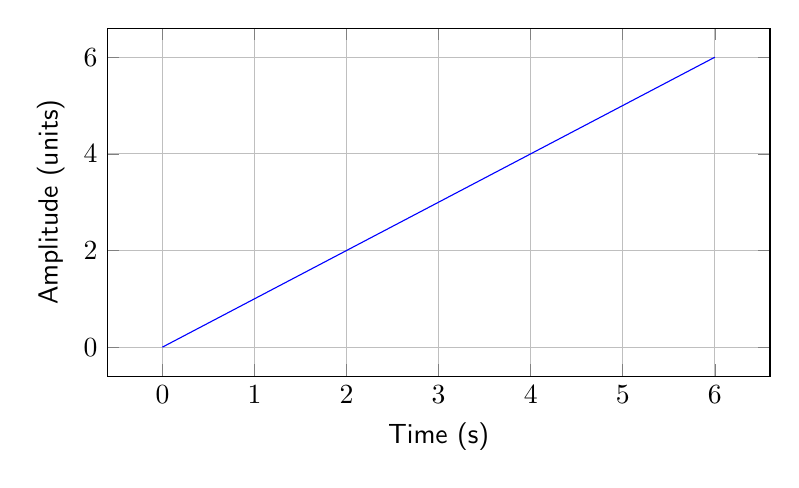
\begin{tikzpicture}
        \begin{axis}[
            xlabel={Time (s)},
            ylabel={Amplitude (units)},
            grid=major,
            width=10cm,
            height=6cm
        ]
        \addplot[
            domain=0:6,
            samples=100,
            color=blue
        ]{x};
        \end{axis}
    \end{tikzpicture}
    \caption{Amplitude as a function of time, demonstrating a linear increase.}
    \label{fig:time_vs_amplitude}
\end{figure}
Figure~\ref{fig:time_vs_amplitude} shows a simple example of amplitude varying linearly with time. This kind of plot is useful for illustrating the basic relationship between time and a measured quantity in controlled experiments \cite{kothari2004research}, \cite{weste2016cmosvlsi}, \cite{ozcan2016cognitive}, \cite{waldron2003generalized}, \cite{maedche2005ontology}. 

\chapter{\uppercase{Result Analysis and Discussion}}
\begin{figure}[h]
    \centering
    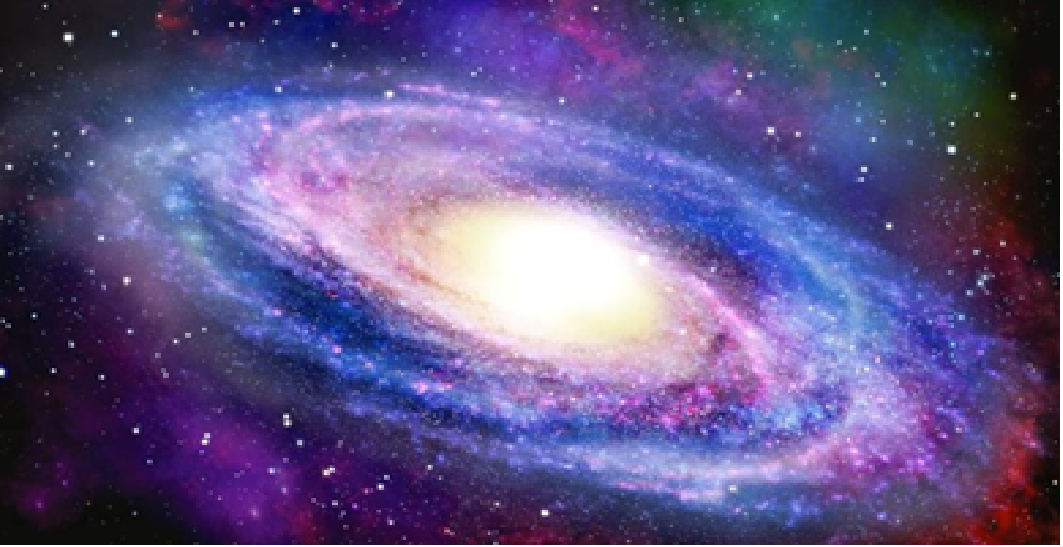
\includegraphics[width=0.5\linewidth]{images/image1.png}
    \caption{Sample picture of universe }
    \label{fig:universe}
\end{figure}
\begin{figure}[h!]
    \centering
    % Left image (a)
    \begin{subfigure}[b]{0.45\linewidth}
        \centering
        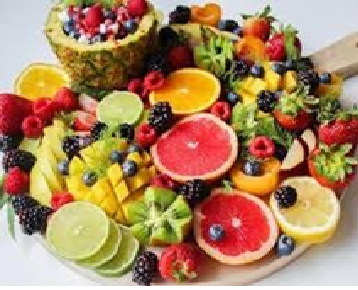
\includegraphics[width=\textwidth]{images/image2.png} % replace with your image filename
        \caption{Fruits containing 'A' vitamin}
        \label{fig:fruitsA}
    \end{subfigure}
    \hfill
    % Right image (b)
    \begin{subfigure}[b]{0.45\linewidth}
        \centering
        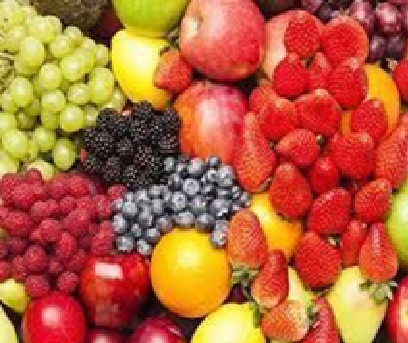
\includegraphics[width=\textwidth]{images/image3.png} % replace with your image filename
        \caption{Fruits containing 'C' vitamin}
        \label{fig:fruitsC}
    \end{subfigure}
    
    \caption{Commonly available fruits}
    \label{fig:common_fruits}
\end{figure}
\chapter{\uppercase{Conclusions and Future Enhancements}}
The conclusion will need to have several elements, including:

\begin{itemize}
    \item A brief summary, just a few paragraphs, of your key findings, related back to what you expected to see (essential);
    \item The conclusions which you have drawn from your research (essential);
    \item Why your research is important for researchers and practitioners (essential);
    \item Recommendations for future research (strongly recommended, verging on essential);
    \item Recommendations for practitioners (strongly recommended in management and business courses and some other areas, so check with your supervisor whether this will be expected); and a final paragraph rounding off your dissertation or thesis.
\end{itemize}

In any research-oriented work, references and citations play a crucial role in establishing the credibility and reliability of the study. Citations are used within the main body of the report to acknowledge the original sources of ideas, theories, methodologies, and results that have informed the research. They allow the reader to trace the origin of information, verify claims, and gain deeper insight into the background literature\cite{waldron2003generalized}.

References, on the other hand, are listed at the end of the dissertation or thesis. They provide the complete bibliographic details of all the sources cited in the text. A well-structured reference list demonstrates the breadth and depth of the literature consulted during the research process. It also helps future researchers to locate relevant works more efficiently\cite{kothari2004research}.

In this report, references have been cited in accordance with standard academic practice. Each in-text citation corresponds to a detailed entry in the reference list. Sources include journal papers, conference proceedings, books, technical reports, and reputable online resources. The citation style followed (e.g., IEEE, APA, or any style recommended by the institute) ensures uniformity and consistency throughout the document\cite{haykin2005cognitive}.


%------ Bibliography ----------------------------------------
%\bibliographystyle{apalike} 
\bibliographystyle{apalike} % Or another desired style like unsrt, abbrv, alpha
\bibliography{mali.bib} % Replace with your .bib filename (without .bib extension)
%\printbibliography [title={REFERENCES}{\centering}]



%------ Appendices ----------------------------------------
\newpage
\begin{center}
\vspace*{5in}
 {\Large \textbf{APPENDICES}}  
\end{center}

\newpage
\begin{center}
 {\Large \textbf{Appendix A}} \\\vspace*{0.5 cm}
 {\Large \textbf{'Log' Table}}
\end{center}
 \begin{center}
\begin{tabular}{|c|c|}
\hline
\textbf{Number} & \textbf{log\textsubscript{10}(Number)} \\
\hline
1 & 0.0000 \\
2 & 0.3010 \\
3 & 0.4771 \\
4 & 0.6021 \\
5 & 0.6990 \\
6 & 0.7782 \\
7 & 0.8451 \\
8 & 0.9031 \\
9 & 0.9542 \\
10 & 1.0000 \\
\hline
\end{tabular}
\end{center}

\newpage
\begin{center}
 {\Large \textbf{Appendix A}} \\\vspace*{0.5 cm}
 {\Large \textbf{SAMPLE CODE}}
 
\end{center}
\begin{lstlisting}
/* C or C++ programming **/
#include <iostream>
using namespace std;
int main() {
    int a = 5, b = 10;
    cout << "Before swap: a = " << a << ", b = " << b << endl;
    int temp = a;
    a = b;
    b = temp;
    cout << "After swap: a = " << a << ", b = " << b << endl;
    return 0;
}

/* Java programming **/
public class SwapNumbers {
    public static void main(String[] args) {
        int a = 5, b = 10;
        System.out.println("Before swap: a = " + a + ", b = " + b);
        int temp = a;
        a = b;
        b = temp;
        System.out.println("After swap: a = " + a + ", b = " + b);
    }
}

/* Python programming **/
a = 5
b = 10
print(f"Before swap: a = {a}, b = {b}")
a, b = b, a  # Pythonic swap
print(f"After swap: a = {a}, b = {b}")

/* Javascript programming **/
let a = 5, b = 10;
console.log(`Before swap: a = ${a}, b = ${b}`);
let temp = a;
a = b;
b = temp;
console.log(`After swap: a = ${a}, b = ${b}`);
\end{lstlisting}
%----------------------------------------------------------------- 

%\section{Introduction}
%\printbibliography

\end{document}
